\documentclass[tikz,border=6pt]{standalone}
\usepackage{amsmath,amssymb,mathtools,physics,bm,nicefrac,wasysym}
\usepackage{xcolor}

\definecolor{colone}{RGB}{180,60,60}
\definecolor{coltwo}{RGB}{60,110,180}
\definecolor{colthree}{RGB}{60,140,80}

\definecolor{accent}{HTML}{A13D2C}
\definecolor{accent2}{HTML}{2B5F6B}
\definecolor{muted}{HTML}{5A564F}
\definecolor{panel}{HTML}{F8F6F0}
\definecolor{linecol}{HTML}{D8D2C4}
\definecolor{ink}{HTML}{1E1C1A}
\definecolor{astroblue}{HTML}{1B4F72}
\definecolor{astrodark}{HTML}{17202A}
\definecolor{sunyellow}{HTML}{E8A33D}

\usetikzlibrary{calc,arrows.meta,positioning,decorations.pathreplacing,decorations.markings,angles,quotes,shapes.geometric}
\usepackage{tikz-3dplot}

\newcommand{\vecr}{\vec r}
\newcommand{\vecL}{\vec L}
\newcommand{\vecA}{\vec A}
\newcommand{\vecf}{\vec f}
\newcommand{\vecF}{\vec F}
\newcommand{\vecp}{\vec p}
\newcommand{\avg}[1]{\left\langle #1\right\rangle}
\newcommand{\vecx}{\vec x}
\newcommand{\hatn}{\hat n}
\newcommand{\rhat}{\hat r}
\newcommand{\phihat}{\hat\phi}
\newcommand{\thetahat}{\hat\theta}
\newcommand{\note}[1]{\textcolor{blue!60!black}{\textit{[#1]}}}

% Astronomical acronyms
\newcommand{\LST}{\mathrm{LST}}
\newcommand{\GST}{\mathrm{GST}}
\newcommand{\GMST}{\mathrm{GMST}}
\newcommand{\GAST}{\mathrm{GAST}}
\newcommand{\LMST}{\mathrm{LMST}}
\newcommand{\LAST}{\mathrm{LAST}}
\newcommand{\UT}{\mathrm{UT}}
\newcommand{\UTC}{\mathrm{UTC}}
\newcommand{\TAI}{\mathrm{TAI}}
\newcommand{\TT}{\mathrm{TT}}
\newcommand{\TDB}{\mathrm{TDB}}
\newcommand{\JD}{\mathrm{JD}}
\newcommand{\MJD}{\mathrm{MJD}}
\newcommand{\EoT}{\mathrm{EoT}}
\newcommand{\SNR}{\mathrm{SNR}}
\newcommand{\RON}{\mathrm{RON}}

% Helper commands for specific diagrams
\newcommand{\midlinelabel}[3]{
    \node (midlabel) at ($ (#1)!.5!(#2) $) {#3};
    \draw[stealth-] (#1) --  (midlabel);
    \draw[-stealth] (midlabel) -- (#2);
}
\newcommand{\midlinelabell}[3]{
    \node[fill = white, inner sep = 0.2pt, outer sep=3pt] (midlabel) at ($ (#1)!.5!(#2) $) {#3};
    \draw[stealth-] (#1) --  (midlabel);
    \draw[-stealth] (midlabel) -- (#2);
}
\newcommand{\midlinelabelll}[3]{
    \node[fill = white, inner sep = 0.2pt, outer sep=3pt,scale=0.6] (midlabel) at ($ (#1)!.5!(#2) $) {#3};
    \draw[stealth-] (#1) --  (midlabel);
    \draw[-stealth] (midlabel) -- (#2);
}



\begin{document}
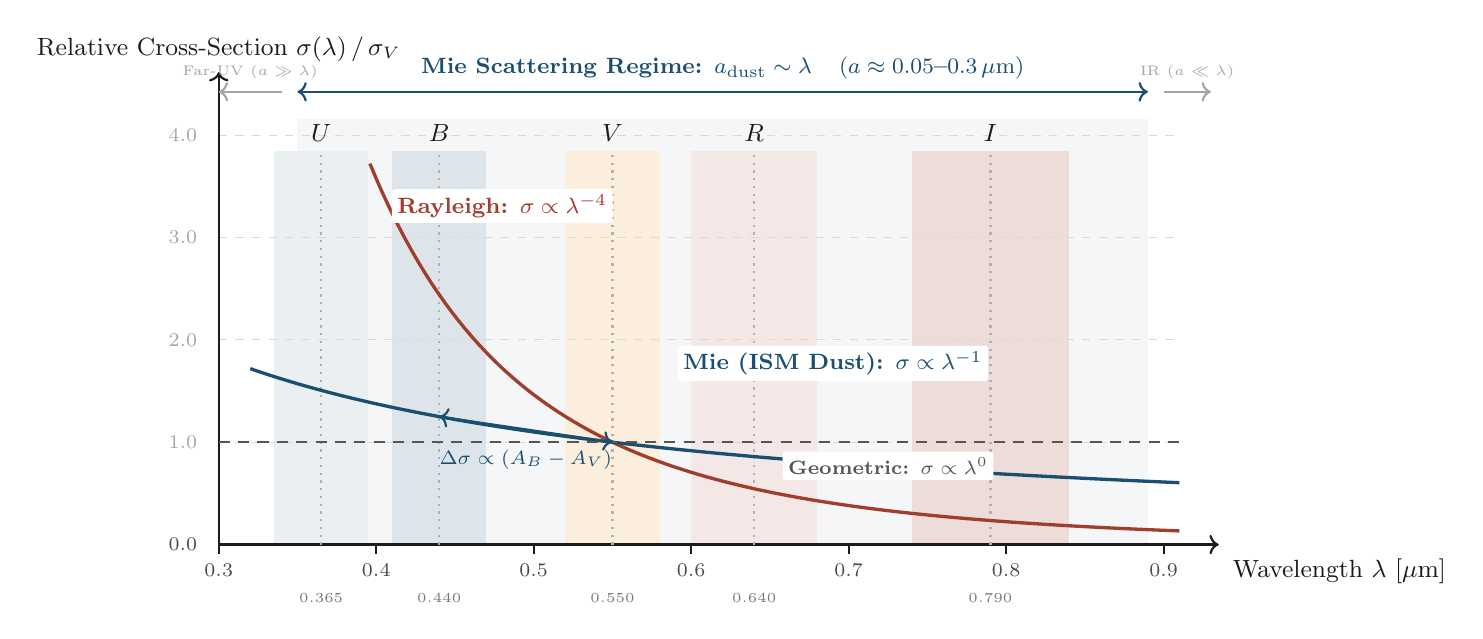
\begin{tikzpicture}[
		scale=1.0,
		declare function={
			wl(\x) = 0.30 + \x/20.0;
			rayleigh(\x) = 1.3 * ((0.55 / wl(\x))^4);
			mie(\x) = 1.3 * (0.55 / wl(\x));
			geom(\x) = 1.3 * 1.0;
		}
	]
		% Regime demarker background band
		\fill[astroblue!5] (1.0,0) rectangle (11.8,5.4);

		% Background passband shading
		\fill[astroblue!9] (0.7,0) rectangle (1.9,5.0); % U band region
		\fill[astroblue!15] (2.2,0) rectangle (3.4,5.0); % B band region
		\fill[sunyellow!18] (4.4,0) rectangle (5.6,5.0); % V band region
		\fill[accent!12] (6.0,0) rectangle (7.6,5.0); % R band region
		\fill[accent!18] (8.8,0) rectangle (10.8,5.0); % I band region

		% Grid lines
		\foreach \yval/\ylabel in {1.3/1.0, 2.6/2.0, 3.9/3.0, 5.2/4.0} {
			\draw[dashed, gray!30, thin] (0,\yval) -- (12.2,\yval);
			\node[gray!70, font=\scriptsize, anchor=east] at (-0.15,\yval) {$\ylabel$};
		}

		% Axes
		\draw[->, thick, ink] (0,0) -- (12.7,0) node[below right=2pt, font=\small] {Wavelength $\lambda$ [$\mu\mathrm{m}$]};
		\draw[->, thick, ink] (0,0) -- (0,6.0) node[above, font=\small] {Relative Cross-Section $\sigma(\lambda)\,/\,\sigma_V$};

		% X-axis ticks
		\foreach \l/\xpos in {0.3/0, 0.4/2.0, 0.5/4.0, 0.6/6.0, 0.7/8.0, 0.8/10.0, 0.9/12.0} {
			\draw[thick, ink] (\xpos,0) -- (\xpos,-0.12);
			\node[ink!80, font=\scriptsize, below] at (\xpos,-0.12) {$\l$};
		}
		\node[ink!80, font=\scriptsize, anchor=east] at (-0.15,0) {$0.0$};

		% Passband center lines & labels
		\foreach \wl/\band/\xpos in {0.365/U/1.30, 0.440/B/2.80, 0.550/V/5.00, 0.640/R/6.80, 0.790/I/9.80} {
			\draw[dotted, thick, ink!35] (\xpos,0) -- (\xpos,5.0);
			\node[ink, font=\small\bfseries, above] at (\xpos,5.0) {$\band$};
			\node[ink!60, font=\tiny, below=14pt] at (\xpos,0) {$\wl$};
		}

		% Regime demarkers (top bar)
		\draw[<->, thick, astroblue] (1.0, 5.75) -- (11.8, 5.75);
		\node[astroblue, font=\footnotesize\bfseries, above=1pt] at (6.4, 5.75) {Mie Scattering Regime: $a_{\rm dust} \sim \lambda \quad (a \approx 0.05\text{--}0.3\,\mu\mathrm{m})$};
		\draw[->, thick, gray!70] (0.8, 5.75) -- (0.0, 5.75);
		\node[gray!70, font=\tiny, above=1pt] at (0.4, 5.75) {Far-UV ($a \gg \lambda$)};
		\draw[->, thick, gray!70] (12.0, 5.75) -- (12.6, 5.75);
		\node[gray!70, font=\tiny, above=1pt] at (12.3, 5.75) {IR ($a \ll \lambda$)};

		% Curves
		\draw[very thick, accent, domain=1.92:12.2, samples=120] plot (\x, {rayleigh(\x)});
		\draw[very thick, astroblue, domain=0.4:12.2, samples=100] plot (\x, {mie(\x)});
		\draw[thick, muted, dash pattern=on 4pt off 3pt, domain=0:12.2] plot (\x, {geom(\x)});

		% Curve labels
		\node[accent, font=\footnotesize\bfseries, fill=white, inner sep=2pt, rounded corners=1pt] at (3.6,4.3) {Rayleigh: $\sigma \propto \lambda^{-4}$};
		\node[astroblue, font=\footnotesize\bfseries, fill=white, inner sep=2pt, rounded corners=1pt] at (7.8,2.3) {Mie (ISM Dust): $\sigma \propto \lambda^{-1}$};
		\node[muted, font=\scriptsize\bfseries, fill=white, inner sep=2pt, rounded corners=1pt] at (8.5,1.0) {Geometric: $\sigma \propto \lambda^0$};

		% Differential extinction indicator (A_B - A_V)
		\draw[<->, thick, astroblue] (2.8,1.625) -- (5.0,1.30);
		\node[astroblue, font=\scriptsize\bfseries, below=2pt] at (3.9,1.4) {$\Delta\sigma \propto (A_B - A_V)$};
	\end{tikzpicture}
\end{document}
